\section{Kinematics}

Kinematics is the study of motion. In this chapter, we define three useful kinematic quantities, displacement, velocity and acceleration, and use these terms to discuss the motion of an object.

\subsection{kinematic quantities}

\subsubsection{displacement \& distance}

in everyday language, we talk about the \keypoint{distance} travelled by an object, which usually refers to the length travelled by an object without considering in what direction it moves

to fully describe position of an object, we also need specify where it moves

\begin{ilight}
	we define \keypoint{displacement} as the distance moved by an object in a specific direction\index{displacement}
\end{ilight}

\cmt displacement and distance are measured in metres, or any reasonable length units

\cmt displacement is a vector quantity, while distance is a scalar

\cmt displacement is the \emph{straight-line} distance pointing from starting point towards end point

even if actual path taken is curved, displacement is always the straight-line distance

\begin{figure}[!ht]
	\centering
	\begin{tikzpicture}[scale=1]
%	\draw[step=0.5] (0,0) grid (5,5);
	 \draw[thick, dashed,->] (0,0) node[below]{start} [out=150, in=140] to (0.5,2) [out=-40, in=210] to (2.5,4) [out=30, in=185] to (4,3) [out=-5, in=160] to (5.5,4) [out=-20, in=55] to (5,2) node[right]{end};
	 \draw[thick, blue, ->] (0,0) -- (5,2) ;
	 \node[note] at (0.6,2.6) {distance};
	 \node[note] at (3.2,0.5) {displacement};
	 \draw (5.7,3) --++ (1,0.6) node[right] {actual path taken};
	 \draw (4,1.55) --++ (2.2,-0.4) node[right] {straight-line connector};
	\end{tikzpicture}
	
	\caption*{difference between displacement and distance}
\end{figure}


\example{An athlete is running around a circular track of radius 60 m. When he completes one lap, what is the distance moved out? What about his displacement?}

\sol distance moved is the perimeter of the circle: $s = 2\pi r = 2\pi\times 60 \approx 380 \text{ m}$

athlete returns to same starting point after one lap, so displacement is zero \eoe

\begin{wrapfigure}{r}{0.4\textwidth}
%	\vspace*{-12pt}
	\centering
	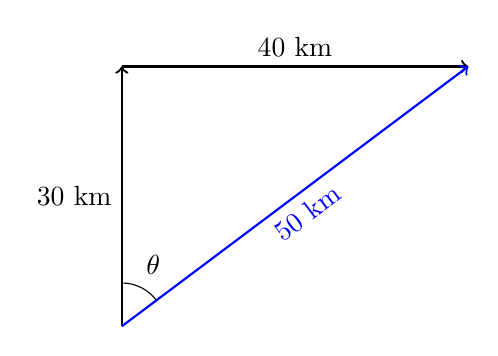
\begin{tikzpicture}[scale=1.1]
	\draw[thick,->] (0,0) -- (0,3) node[midway, left]{30 km};
	\draw[thick,->] (0,3) -- (4,3) node[midway, above]{40 km};
	\draw[thick,blue,->] (0,0) -- (4,3) node[midway, below, rotate=36.89]{50 km};
	\draw (0,0.5) arc(90:36.89:0.5);
	\node at (63:0.8) {$\theta$};
	\end{tikzpicture}
	\vspace*{-16pt}
\end{wrapfigure}

\example{A ship travels 30 km north, takes a right, and then travels 40 km east to reach its destination. Compare the distance and the displacement travelled.}

\sol sum of all lengths gives distance: $30+40 = 70 \text{ km}$

displacement vector is shown on the graph

$\text{magnitude of displacement} = \sqrt{30^2 + 40^2} = 50 \text{ km}$

it is at an angle of $\theta = \tan^{-1}\frac{40}{30} \approx 53^\circ$ east of north \eoe



\subsubsection{velocity \& speed}

displacement of a moving object may change with respect to time

an object is moving fast if it has a large change in displacement during a given time interval

\begin{ilight}
	change in displacement per unit time is called the \keypoint{velocity} of the object\index{velocity}: $\boxed{v=\frac{\Delta s}{\Delta t}}$
\end{ilight}

\cmt SI unit of measurement for velocity: $[v]= \mps$

\cmt velocity is a vector quantity

this follows from the fact that displacement is a vector quantity

\cmt for \emph{linear} motion, one shall pick a specific direction as the positive direction

then a negative velocity implies motion in the opposite direction

\cmt it is also common to use \keypoint{speed} to describe how fast an object moves

speed is defined as the change of the distance travelled per unit time

velocity can be thought as speed in a particular direction

\cmt defining equation $v=\frac{\Delta s}{\Delta t}$ gives the \emph{average} value for velocity or speed over an interval $\Delta t$

more precisely: $\boxed{\text{average velocity} = \frac{\text{total displacement}}{\text{time taken}}}$, and $\boxed{\text{average speed} = \frac{\text{total distance}}{\text{time taken}}}$

\eqyskip this should be distinguished from the notion of \emph{instantaneous velocity}

instantaneous velocity is defined as the rate of change in displacement at a particular instant

if we take a very short interval $\Delta t$, as $\Delta t \to 0$, average velocity tends to instantaneous velocity

this is expressed in a compact differential form: $v = \lim_{\Delta t \to 0} \frac{\Delta s}{\Delta t} \ra \boxed{v=\frac{\dd s}{\dd t}} $

\example{A cyclist travels a distance of 3.0 km in 20 minutes. She rests for 15 minutes. She then covers a further distance of 5.1 km in a time of 40 minutes. Calculate the average speed of the cyclist in m s$^{-1}$: (a) during the first 20 minutes of the journey, (b) for the whole journey.}

\sol for the first 20 minutes: $ v = \frac{3.0\times10^3}{20 \times 60} = 2.5 \mps$

\eqyskip for whole journey: $v = \frac{(3.0+0+5.1)\times10^3}{(20+15+40)\times60} = 1.8 \mps $ \eoe

\example{A man walks along a straight road for a distance of 800 m in 5.0 minutes. He then turns around, and walks along the same road for a distance of 280 m in 3.0 minutes. What is the average speed and the average velocity of this man during the 8.0 minutes?}

\sol $\text{total distance travelled} = 800 + 280 = 1080 \text{m}$, so average speed: $v = \frac{1080}{8.0\times60} = 2.25 \mps$

\eqyskip  $\text{change of displacement} = 800 + (-280) = 520 \text{m}$, so average velocity: $v = \frac{520}{8.0\times60} \approx 1.08 \mps$ \eoe

\example{A maglev train travels at an average speed of $60\mps$ from the city centre to the airport, and at $40\mps$ on its return journey over the same distance. What is the average speed of the round-trip? What about the average velocity?}

\sol suppose the distance between airport and city centre is $S$

average speed: $v = \frac{2S}{t_1 + t_2} = \frac{2S}{\frac{S}{60} + \frac{S}{40}} = 48 \mps$

for a round-trip, train returns to same staring position

change in displacement is zero, so average velocity is zero \eoe



\subsubsection{acceleration}

velocity of a moving object may change as well, i.e., objects can speed up or slow down

\begin{ilight}
	change in velocity per unit time is defined as the \keypoint{acceleration}\index{acceleration}: $\boxed{a = \frac{\Delta v}{\Delta t}}$
\end{ilight}

\cmt unit of measurement for acceleration: $[a]= \mpss$

\cmt acceleration is a vector quantity, it has both magnitude and direction

this is because of vector nature of velocity, change in velocity must also have direction

\cmt for \emph{linear} motion, one usually pick direction of initial velocity as positive direction

$a>0$ would imply acceleration in the normal sense, i.e., motion with an increasing speed

$a<0$ would imply deceleration, i.e., motion with a decreasing speed

\cmt when velocity changes, it could be change in magnitude or/and change in direction
\footnote{Acceleration of an object can be considered as the combination of two components. One component is known as the \emph{normal} acceleration or the \emph{centripetal} acceleration, which is at right angle to the velocity and is responsible for the change in direction of motion. The other component is called the \emph{tangential} acceleration, which is parallel to the direction of motion and causes change in magnitude of object's velocity. You will learn more about these in further mechanics.}

for example, for an object moving along a curved path, its velocity is constantly changing direction, so it must have a non-zero acceleration

no acceleration would imply no change in speed and no change in direction of motion

\cmt defining equation $a = \frac{\Delta v}{\Delta t}$ gives average acceleration over time interval $\Delta t$

we can likewise introduce \emph{instantaneous acceleration} as the rate of change in velocity

taking the limit where the time interval $\Delta t \to 0$. we have: $a = \lim_{\Delta t \to 0} \frac{\Delta v}{\Delta t} \ra \boxed{a=\frac{\dd v}{\dd t}} $

\example{A ball hits a barrier at right angles with a speed of $15 \mps$. It makes contact with the barrier for 30 ms and then rebounds with a speed of $12 \mps$. What is the average acceleration during the time of contact?}

\sol note that direction of velocity changed during rebound, so $\Delta v = 15 - (-12) = 27 \mps$

average acceleration: $a = \frac{\Delta v}{\Delta t} = \frac{27}{30 \times 10^{-3}} = 900 \mpss$ \eoe



\subsection{motion graphs}

how one physical quantity changes with another quantity can be visually shown on a \emph{graph}

changes in displacement, velocity or acceleration over time can be shown on \emph{motion graphs}\index{motion graphs}

as we will see, $s$-$t$ graph, $v$-$t$ graph and $a$-$t$ graphs are closely interrelated to one another

\subsubsection{displacement-time graphs}

a displacement-time graph shows an object's position at any given time

\cmt gradient of tangent gives rate of change in displacement

but this is instantaneous velocity, which can be given by $v = \frac{\dd s}{\dd t}$, so we have:

{
	\centering
	
	\eqyskip$ \boxed{\text{velocity} = \text{gradient of $s$-$t$ graph}} $
	
}

\newpage


\example{Describing the motion from the displacement-time graph shown.}

\begin{wrapfigure}{L}{0.36\textwidth}
	\vspace{-24pt}
	\begin{center}
		\begin{tikzpicture}[xscale=1.1,yscale=0.95]
		\draw[<->] (0,3.2)node[left]{s} -- (0,0) -- (4.2,0)node[below]{$t$};
		\draw[blue, thick] plot [smooth] coordinates {(0,0) (.5,.2) (1,.8) (1.5,2.0) (2,2.5) (2.5,2.7) (3.0,2.8) (4,2.8)};
		\node at (.8,1) {$A$};
		\node at (2,2.8) {$B$};
		\node at (3.5,3) {$C$};
		\end{tikzpicture}
	\end{center}
	\vspace{-27pt}
\end{wrapfigure}

	stage $A$: gradient of the graph is increasing, showing that the object is speeding up
		
	stage $B$: gradient starts to decrease, so the object gradually slows down
		
	stage $C$: curve becomes horizontal, gradient becomes zero, means that the object eventually comes to a stop \eoe
	
\begin{wrapfigure}{r}{0.45\textwidth}
	\vspace*{-12pt}
	\centering
	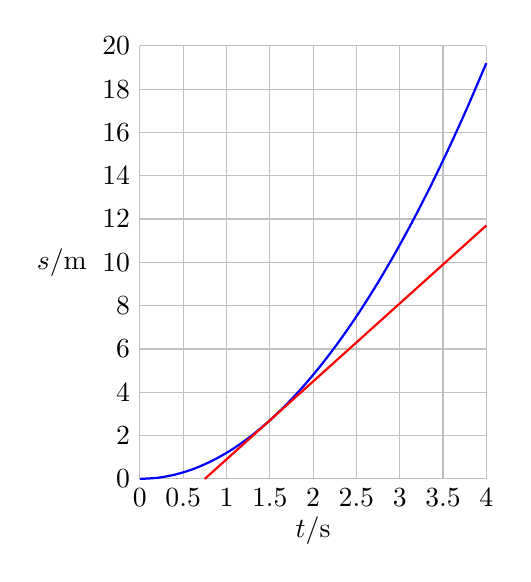
\begin{tikzpicture}[scale=1.1]
		\draw[gray!50,step=0.5] (0,0) grid (4,5);
		\draw[thick, blue,smooth, samples=20, domain=0:4] plot (\x, 0.3*\x*\x);
		\foreach \x in {0,0.5,1,1.5,2,2.5,3,3.5,4} \node[below] at (\x,0){$\x$};
		\foreach \y in {0,2,...,20} \node[left] at (0,\y/4) {$\y$};
		\node at (2,-0.6) {$t$/s};
		\node[left] at (-0.5,2.5) {$s$/m};
		\draw[thick,red] (0.75,0) -- (4,2.925);
	\end{tikzpicture}
	\vspace*{-10pt}
\end{wrapfigure}

\example{The diagram shows the displacement-time graph for a vehicle travelling along a straight road. Use the graph to find, (a) the average velocity during the first 4.0 s of the motion, (b) the velocity of the vehicle \emph{at} time $t=1.5$ s.}

\sol during first 4.0 s, average velocity is

{
	\centering
	
	$ v = \frac{\Delta s}{\Delta t} = \frac{19.2}{4.0} \approx 4.8 \mps$
	
}

to find velocity at $t=1.5$ s, a tangent is drawn

gradient of tangent gives instantaneous velocity:

{
	\centering
	
	$ v = \frac{11.6 - 0}{4.0-0.75} \approx 3.6 \mps $
	
}

\vspace*{-\baselineskip} \eoe

\subsubsection{velocity-time graphs}

a velocity-time graph shows the velocity of a moving object at any instant

\cmt since the rate of change of velocity gives the acceleration, so
\begin{equation*}
\boxed{\text{acceleration} = \text{gradient of $v$-$t$ graph}}
\end{equation*}

\cmt $v$-$t$ graph also gives information about the change in displacement
\begin{equation*}
\boxed{\text{change in displacement} = \text{area under $v$-$t$ graph}}
\end{equation*}

in very short time interval $\Delta t_i$, change in velocity is small so $v(t_i)\approx\text{constant}$ during this time

displacement moved out $\Delta s_i \approx v(t_i) \Delta t_i$, which corresponds to area of a thin rectangle

sum of all these small $\Delta s_i$'s gives total change in displacement over a period of time

now consider the limit where each of the time interval $\Delta t_i \to 0$

total area of these rectangles approximates area bounded by the $v$-$t$ curve and time axis
\footnote{Mathematically, integration is the inverse operation of taking derivatives. By definition $v=\frac{\dd s}{\dd t}$, then it follows naturally that $\Delta s = \int v\dd t$. While the derivative of a given function gives the gradient of tangent at each point on its graph, integrating a function gives the signed area bounded by the graph. The reader may find the formal treatment of this relationship in any calculus textbook.}

\begin{figure}[!ht]
	\noindent\centering
	\begin{minipage}{0.32\linewidth}
	\centering
	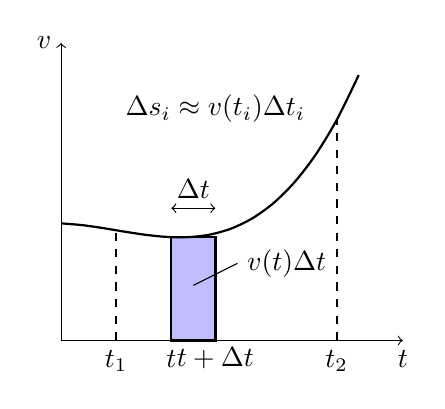
\begin{tikzpicture}[scale=1.4]
	\draw[thick,fill=blue!25] (1.5,0) rectangle (1.9,0.9375);
	\draw (1.7,0.5) -- (2.1,0.7) node[right]{$v(t)\Delta t$};
	\draw[<->] (1.5,1.2) -- (1.9,1.2) node[midway,above]{$\Delta t$};
	\draw[<->] (0.5,2.7) node[left]{$v$} -- (0.5,0) -- (3.6,0) node[below]{$t$};
	\draw [thick,domain=0.5:3.2,samples=15,smooth,variable=\x] plot (\x,{\x*(\x-1)*(\x-2)/6+1});
	\draw[thick,dashed] (1,0) node[below]{$t_1$} -- (1,1);
	\draw[thick,dashed] (3,0) node[below]{$t_2$} -- (3,2);
	\node[below] at (1.5,0) {$t$};
	\node[below] at (1.9,0.02) {$t+\Delta t$};
	\node at (1.9,2.1){$\Delta s_i \approx v(t_i)\Delta t_i$};
	\end{tikzpicture}
	(a) displacement $\Delta s$
	
	in short interval $\Delta t$
	\end{minipage}\hfill
	\begin{minipage}{0.34\linewidth}
		\centering
		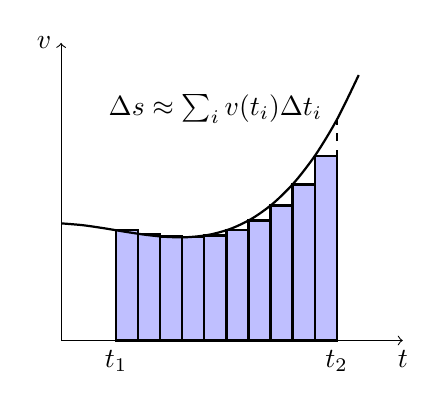
\begin{tikzpicture}[scale=1.4]
		\foreach \x in {1.0,1.2,1.4,...,2.8}
		{ \draw[thick,fill=blue!25] (\x,0) rectangle (\x+.2,{\x*(\x-1)*(\x-2)/6+1});
			}
		\draw[thick,dashed] (1,0) node[below]{$t_1$} -- (1,1);
		\draw[thick,dashed] (3,0) node[below]{$t_2$} -- (3,2);
		\draw[<->] (0.5,2.7) node[left]{$v$} -- (0.5,0) -- (3.6,0) node[below]{$t$};
		\draw [thick,domain=0.5:3.2,samples=15,smooth,variable=\x] plot (\x,{\x*(\x-1)*(\x-2)/6+1});
		\node at (1.9,2.1){$\Delta s \approx \sum_i v(t_i)\Delta t_i$};
		\end{tikzpicture}
		(b) total displacement estimated	
		
		by summing the many $\Delta s_i$'s
	\end{minipage}\hfill
	\begin{minipage}{0.32\linewidth}
		\centering
		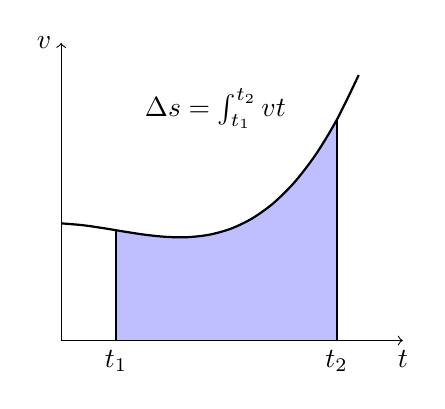
\begin{tikzpicture}[scale=1.4]
		\fill[fill=blue!25] (1,0) -- plot[domain=1:3,samples=15,smooth,variable=\x] (\x,{\x*(\x-1)*(\x-2)/6+1}) -- (3,0) -- cycle;
		\draw[thick] (1,0) node[below]{$t_1$} -- (1,1);
		\draw[thick] (3,0) node[below]{$t_2$} -- (3,2);
		\draw[<->] (0.5,2.7) node[left]{$v$} -- (0.5,0) -- (3.6,0) node[below]{$t$};
		\draw [thick,domain=0.5:3.2,samples=15,smooth,variable=\x] plot (\x,{\x*(\x-1)*(\x-2)/6+1});
		\node at (1.9,2.1){$\Delta s = \int_{t_1}^{t_2} v \dd t$};
		\end{tikzpicture}
		(c) total displacement as
		
		area under $v$-$t$ graph
	\end{minipage}
	\caption*{calculating change in displacement by finding the area under velocity-time graph}\label{fig:area_of_vt}
\end{figure}

\begin{wrapfigure}{r}{0.45\textwidth}
	\vspace*{0pt}
	\centering
	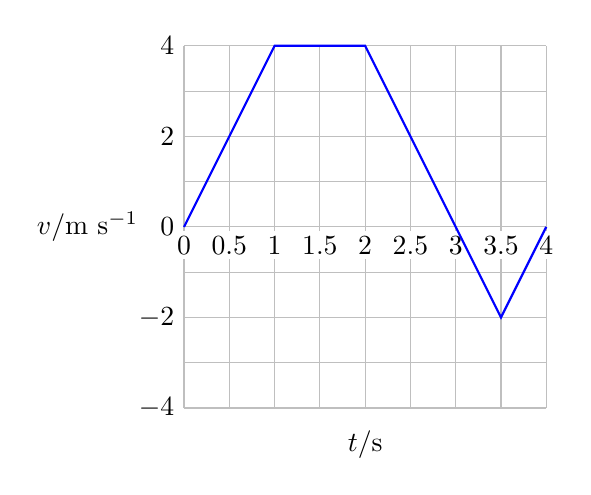
\begin{tikzpicture}[scale=1.15]
	\draw[gray!50,step=0.5] (0,-2) grid (4,2);
	\foreach \x in {0,0.5,1,1.5,2,2.5,3,3.5,4} {
	\draw[white,fill] (\x-0.1,-0.35) rectangle (\x+0.1,-0.05);
	\node[below] at (\x,0){$\x$};
	}
	\foreach \y in {-4,-2,0,2,4} \node[left] at (0,\y/2) {$\y$};
	\draw[blue,thick] (0,0) -- (1,2) -- (2,2) -- (3.5,-1) -- (4,0);
	\node at (2,-2.4) {$t$/s};
	\node[left] at (-0.4,0) {$v$/m s$^{-1}$};
	\end{tikzpicture}
	\vspace*{-16pt}
\end{wrapfigure}


\example{The velocity of a toy car is shown. For the journey shown on the graph, use the graph to find (a) the total distance travelled, and (b) the total displacement travelled.}

\sol distance is estimated using area under $v$-$t$ graph

0$\sim$3.0 s: $s_1 = \frac{1}{2}\times{1.0+3.0}\times4.0 = 8.0 \text{ m}$

3.0$\sim$4.0 s: $s_2 = \frac{1}{2}\times{1.0}\times2.0 = 1.0 \text{ m}$

$\text{total distance} = 8.0 + 1.0 = 9.0 \text{ m}$

$\text{total displacement} = (+8.0) + (-1.0) = 7.0 \text{ m}$ \eoe

\subsubsection{acceleration-time graphs}

one can similarly plot an acceleration-time graph to give the changes in acceleration

\cmt $a$-$t$ graphs can give information about changes in velocity

similar discussions lead to the following conclusion:\footnote{Using area under $a$-$t$ graph to find changes in velocity is not required in the AS-Level physics syllabus. I am putting this in the notes mainly for the completeness of the discussions on motion graphs.}
\begin{equation*}
\boxed{\text{change in velocity} = \text{area under $a$-$t$ graph}}
\end{equation*}

\newpage

relationships between displacement, velocity and acceleration graphs are summarised below

\begin{figure}[!ht]
	\centering
	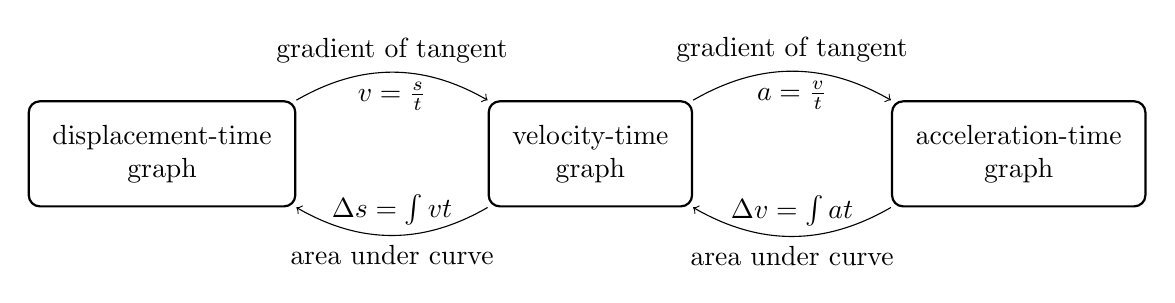
\begin{tikzpicture}[force/.style={align=center,execute at begin node=\setlength{\baselineskip}{1.2em},draw,thick,rounded corners,inner sep=.3cm},scale=0.85]
	
	\node [force] (displacement) at (0,0) {displacement-time\\ graph};
	\node [force] (velocity) at (6.4,0) {velocity-time\\graph};
	\node [force] (acceleration) at (12.8,0) {acceleration-time\\graph};
	
	\draw[->] (displacement.north east) to [bend left] node[midway,above]{gradient of tangent} node[midway,below]{$v=\frac{\dd s}{\dd t}$} (velocity.north west);
	\draw[<-] (displacement.south east) to [bend right] node[midway,below]{area under curve} node[midway,above]{$\Delta s=\int v\dd t$} (velocity.south west);
	\draw[->] (velocity.north east) to [bend left] node[midway,above]{gradient of tangent} node[midway,below]{$a=\frac{\dd v}{\dd t}$} (acceleration.north west);
	\draw[<-] (velocity.south east) to [bend right] node[midway,below]{area under curve} node[midway,above]{$\Delta v=\int a\dd t$} (acceleration.south west);
	\end{tikzpicture}
%	\caption*{relationships between motion graphs}
\end{figure}

\example{Given the displacement-time graph as shown, check yourself that this $s$-$t$ graph leads to the velocity-time graph and the acceleration-time graph shown.}

\begin{figure}[ht]
	\centering
	\begin{minipage}{0.3\textwidth}
		\centering
		\begin{tikzpicture}[xscale=0.6,yscale=0.9]
		\draw[<->] (0,2) node[left]{$s$} -- (0,0) -- (7,0) node[below]{$t$};
		\draw (0,0) -- (0,-2);
		\draw [thick,blue,domain=0:6.7,smooth] plot (\x, {1.6*sin(\x r)});
		\end{tikzpicture}
	\end{minipage}\hfil
	\begin{minipage}{0.3\textwidth}
		\centering
		\begin{tikzpicture}[xscale=0.6,yscale=0.9]
		\draw[<->] (0,2) node[left]{$v$} -- (0,0) -- (7,0) node[below]{$t$};
		\draw (0,0) -- (0,-2);
		\draw [thick,red,domain=0:6.7,smooth] plot (\x, {1.6*cos(\x r)});
		\end{tikzpicture}
	\end{minipage}\hfil
	\begin{minipage}{0.3\textwidth}
		\centering
		\begin{tikzpicture}[xscale=0.6,yscale=0.9]
		\draw[<->] (0,2) node[left]{$a$} -- (0,0) -- (7,0) node[below]{$t$};
		\draw (0,0) -- (0,-2);
		\draw [thick,red,domain=0:6.7,smooth] plot (\x, {-1.6*sin(\x r)});
		\end{tikzpicture}
	\end{minipage}
\end{figure}

\example{Given the velocity-time graph as shown, check yourself that this $v$-$t$ graph leads to the displacement-time graph as shown.}\label{ex-vgraph}

\begin{figure}[ht]
	\centering
	\begin{minipage}{0.45\textwidth}
		\centering
		\begin{tikzpicture}[xscale=0.8,yscale=1.1]
		\draw[<->] (0,3) node[left]{$v$} -- (0,0) -- (7,0) node[below]{$t$};
		\draw [thick,blue] (0,0) -- (2,2.5) -- (4,2.5) [out=-75,in=180] to (6,0);
		\draw[dashed] (2,0) -- (2,2.5)  (4,0) -- (4,2.5);
		\end{tikzpicture}
	\end{minipage}\hfil
	\begin{minipage}{0.45\textwidth}
		\centering
		\begin{tikzpicture}[xscale=0.8,yscale=1.1]
		\draw[<->] (0,3) node[left]{$s$} -- (0,0) -- (7,0) node[below]{$t$};
		\draw [thick,red,domain=0:2] plot (\x,0.2*\x*\x);
		\draw [thick,red] (2,0.8) -- (4,2.4);
		\draw [thick,red,domain=4:6] plot (\x,{2.4+0.8*(1-exp(-2.5*\x+2.5*4))/2.5});
		\draw[dashed] (2,0) -- (2,0.8)  (4,0) -- (4,2.4);
		\end{tikzpicture}
	\end{minipage}
\end{figure}





\subsection{linear motion with constant velocity}

let's look at the simplest kind of motion

that is, an object moving at constant speed in a straight line: $v=\text{constant}$

the equations of motion are straightforward:
\begin{equation}
	a=0 \qquad \boxed{s=vt}\footnote{It is implicitly assumed that the motion starts from the origin with respect to which displacement is defined. More generically, we should write: $s = s_0 + vt$, where $s_0$ is the initial displacement.}
\end{equation}

\begin{figure}[htp]
	\centering
	\begin{minipage}{0.32\textwidth}
		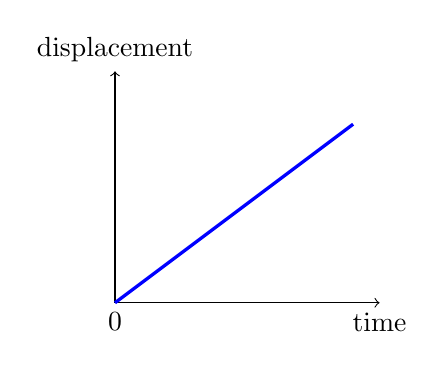
\begin{tikzpicture}[scale=0.84]
		\draw [<->] (0,3.5) node[above] {displacement} -- (0,0) node[below]{0} -- (4,0) node[below] {time};
		\draw[very thick,blue] (0,0) -- (3.6,2.7);
		\end{tikzpicture}
	\end{minipage}\hfill
	\begin{minipage}{0.32\textwidth}
		\begin{tikzpicture}[scale=0.84]
		\draw [<->] (0,3.5) node[above] {velocity} -- (0,2.5) node[left]{$v$} -- (0,0) node[below]{0} -- (4,0) node[below] {time};
		\draw[very thick,blue] (0,2.5) -- (3.6,2.5);
		\draw[dashed] (3,2.5) -- (3,0) node[below]{$t$};
		\end{tikzpicture}
	\end{minipage}\hfill
	\begin{minipage}{0.32\textwidth}
		\begin{tikzpicture}[scale=0.84]
		\draw [<->] (0,3.5) node[above] {acceleration} -- (0,0) node[below]{0} -- (4,0) node[below] {time};
		\draw[very thick,blue] (0,0.01) -- (3.6,0.01);
		\end{tikzpicture}
	\end{minipage}
	\caption*{motion graphs for linear motion at constant velocity}
\end{figure}



\subsection{linear motion with constant acceleration}

the second simplest type of motion is a linear motion with acceleration $a=\text{constant}$

\begin{figure}[htp]
	\centering
	\begin{minipage}{0.32\textwidth}
		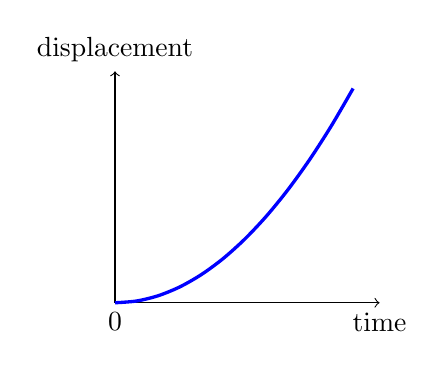
\begin{tikzpicture}[scale=0.84]
		\draw [<->] (0,3.5) node[above] {displacement} -- (0,0) node[below]{0} -- (4,0) node[below] {time};
		\draw [very thick,blue,domain=0:3.6,samples=12,smooth,variable=\x] plot (\x,{\x*\x/4});
		\end{tikzpicture}
	\end{minipage}\hfill
	\begin{minipage}{0.32\textwidth}
		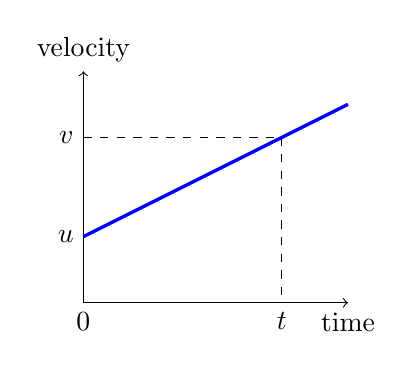
\begin{tikzpicture}[scale=0.84]
		\draw [<->] (0,3.5) node[above] {velocity} -- (0,1) node[left]{$u$} -- (0,0) node[below]{0} -- (4,0) node[below]{time};
		\draw[very thick,blue] (0,1) -- (4,3);
		\draw[dashed] (0,2.5) node[left]{$v$}  -- (3,2.5);
		\draw[dashed] (3,2.5) -- (3,0) node[below]{$t$};
		\end{tikzpicture}
	\end{minipage}\hfill
	\begin{minipage}{0.32\textwidth}
		\begin{tikzpicture}[scale=0.84]
		\draw [<->] (0,3.5) node[above] {acceleration} -- (0,2.5) node[left]{$a$} -- (0,0) node[below]{0} -- (4,0) node[below] {time};
		\draw[very thick,blue] (0,2.5) -- (3.6,2.5);
		\end{tikzpicture}
	\end{minipage}
	\caption*{motion graphs for linear motion at constant acceleration}\label{fig:const_a_graph}
\end{figure}

\subsubsection{equations of motion}

during a time interval $t$, suppose velocity changes from initial value $u$ to final value $v$

from the defining equation of acceleration $a=\frac{\Delta v}{\Delta t} = \frac{v-u}{t}$, we get
\begin{equation}\label{eqn:const_a_eq1}
\boxed{v=u+at}
\footnote{Proof with calculus: $\dd v = a \dd t \ra \Delta v = \int_u^v \dd v = \int_0^t a\dd t \ra v-u=at \ra v=u+at$}
\end{equation}

to find total displacement travelled, we compute the area under the $v$-$t$ graph
\begin{equation}\label{eqn:const_a_eq2}
	\boxed{s=\frac{1}{2}(u+v)t}
\end{equation}
for which we can interpret $\bar{v}=\frac{1}{2}(u+v)$ as the average velocity during that time

plug \eqref{eqn:const_a_eq1} into \eqref{eqn:const_a_eq2}, we find an expression for the displacement travelled in terms of $u$ and $a$:
\begin{equation}\label{eqn:const_a_eq3}
	\boxed{s = ut + \frac{1}{2}at^2}
	\footnote{Proof with calculus: $\dd s = v \dd t \ra \Delta s = \int_0^s \dd s = \int_0^t v\dd t \ra s = \int_0^t (u+at)\dd t = \big(ut+\frac{1}{2}at^2\big)\bigg|_0^t \ra s = ut + \frac{1}{2}at^2$}
	\footnote{Equation \eqref{eqn:const_a_eq3} assumes a zero initial displacement at $t=0$. If there is a non-zero initial displacement, one should write $s = s_0 + ut + \frac{1}{2}at^2$. Similar discussion applies to equation \eqref{eqn:const_a_eq2}.}
\end{equation}

this shows the displacement $s$ is a quadratic function in time $t$

this is consistent with the parabolic shape of the $s$-$t$ graph shown

we can also eliminate the time variable $t$ to derive one last equation

from \eqref{eqn:const_a_eq1} we have $t=\frac{v-u}{a}$, substitute this into \eqref{eqn:const_a_eq2}, we find
\begin{equation}\label{eqn:const_a_eq4}
	s=\frac{1}{2}(u+v)\times\frac{v-u}{a} \RA \boxed{2as = v^2 - u^2}
\end{equation}

\example{A car starts from rest and accelerates uniformly at 5.0\mpss for 6.0 s. (a) How fast is the car travelling at $t=8.0$ s? (b) What is the distance travelled by the car in this time?}

\solc\begin{equation*}
v=u+at \RA v = 0 + 5.0\times 6.0 = 30 \mps
\end{equation*}
\begin{equation*}
s=ut+\frac{1}{2}at^2 \RA s= 0+\frac{1}{2}\times5.0\times6.0^2 = 90 \text{ m} \teoe
\end{equation*}

\example{A car is travelling at 30\mps. A hazard appears in front of the car, and the driver takes immediate action to stop the car. When brakes are applied, deceleration of the car is 5.0\mpss. What is the braking distance?}

\solc\begin{equation*}
2as=v^2-u^2 \RA s = \frac{v^2-u^2}{2a} = \frac{0^2 - 30^2}{2\times(-5.0)} = 90 \text{ m} \teoe
\end{equation*}

\example{At the instant the traffic light turns green, a motorcycle waiting at the stop line starts with a constant acceleration of $2.0 \mpss$. At the same instant, a truck at a constant speed of $16 \mps$ overtakes and passes the motorcycle. How far beyond the stop line will the motorcycle overtake the truck?}

\sol suppose overtake occurs at time $t$ after motorcycle starts to accelerate

distance travelled by motorcycle: $s_m = u_mt + \frac{1}{2}at^2  \RA s_m = 0 + \frac{1}{2}\times 2.0 \times t^2$

distance travelled by truck: $s_t = v_t t \RA s_t = 16t$

overtake when $s_m = s_t \RA \frac{1}{2}\times 2.0 \times t^2 = 16 t \RA t=16 \text{ s}$

substitute $t$ into either $s_m$ or $s_t$, one finds distance travelled: $s = 256 \text{ m}$ \eoe




\subsubsection{free fall}\label{ch_freefall}

a typical example of uniformly accelerated motion is the free fall\index{free fall}

everything has the tendency to fall towards ground due to earth's gravity

in this section, we assume that effects of air resistance are negligible

acceleration of free fall is then a constant $a=g$, regardless of mass of falling object\footnote{The reason for this constant acceleration of free fall will be elaborated in $\S$\ref{ch_weight}.}

\cmt near surface of earth, value of acceleration of free fall: $g\approx9.81\mpss$

value of $g$ could be different on a different planet

\cmt for a freely-falling object released from rest, its velocity increases with time as
\begin{equation*}
	v=u+at = 0 + gt \RA v = gt
\end{equation*}

the distance it has fallen from the point of release is
\begin{equation*}
s=ut+\frac{1}{2} at^2 = 0\cdot t + \frac{1}{2}gt^2 \RA s=\frac{1}{2}gt^2
\end{equation*}

\example{An object is released from rest from a height of $h=24$ m and falls freely under gravity. Air resistance is negligible. (a) How long does it take to hit the ground? (b) What is its speed when hitting the ground?}

\solc\begin{equation*}
h = \frac{1}{2}gt^2 \RA t = \sqrt{\frac{2h}{g}} = \sqrt{\frac{2\times24}{9.81}} \approx 2.21 \text{ s}
\end{equation*}
\begin{equation*}
v = gt = 9.81 \times 2.21 \approx 21.7 \mps \teoe
\end{equation*}

\example{A photograph is taken for a small particle falling from rest. The photograph is taken at 0.400 s after the object is released. Since the particle is still moving when the photograph is being taken, the image is blurred. The blurred part is found to have a length of 20.8 cm. What is time of exposure for the photograph?}

\sol from $t=0$ to right before photo is taken: 

{
	\centering
	
	$s_1 = \frac{1}{2}gt_1^2 = \frac{1}{2}\times9.81\times0.400^2 \approx 0.785 \text{ m}$
	
}

from $t=0$ to right after photo has been taken: 

{
	\centering
	
	$s_2 = s_1 + \Delta s = \frac{1}{2}gt^2_2 \RA t_2 = \sqrt{\frac{2(s_1+\Delta s)}{g}} = \sqrt{\frac{2\times(0.785+0.208)}{9.81}} \approx 0.450 \text{ s}$
	
}

time of exposure: $\Delta t = t_2 - t_1 = 0.450 - 0.400 \approx 0.050 \text{ s}$ \eoe



\subsubsection{upward projection}

like a freely-falling object, an object tossed upwards experiences the same constant downward acceleration $a=g\approx9.81\mpss$ as long as resistive forces can be ignored

note that initial velocity $u$ is upwards, but acceleration $a$ is downwards
so we will have different signs for $u$ and $a$ in the equations

conventionally, positive direction is taken as same direction as initial velocity

in our case, positive direction is upwards, the acceleration is then negative $a=-g$

so the velocity-time relation and displacement-time relation are
\begin{equation*}
v = u - gt \quad \quad s = ut - \frac{1}{2}gt^2
\end{equation*}

\begin{figure}[ht]
	\centering
	\begin{minipage}{0.45\textwidth}
		\centering
		\begin{tikzpicture}[xscale=1.2]
		\draw[->] (0,-3) -- (0,3) node[left]{$v$};
		\draw[->] (0,0) -- (5,0) node[below]{$t$};
		\draw[thick,blue] (0,1.8) -- (5,-2.7);
		\draw (0.8,1.2) --++ (1,0.8) node[above,note]{object is moving\\ upwards ($v>0$)};
		\draw (2,0.05) --++ (1.2,0.4) node[above,note]{object at maximum\\height ($v=0$)};
		\draw (3.2,-1.2) --++ (-1,-0.6) node[below,note]{object is moving\\downwards ($v<0$)};
		\end{tikzpicture}
	\end{minipage}\hfil
	\centering
	\begin{minipage}{0.45\textwidth}
		\centering
		\begin{tikzpicture}[xscale=1.2]
		\draw[->] (0,-3) -- (0,3) node[left]{$s$};
		\draw[->] (0,0) -- (5,0) node[below]{$t$};
		\draw[thick,blue,domain=0:5,smooth] plot (\x,{-0.5*\x*(\x-4)});
		\draw (2.05,2.05) --++ (1,0.4) node[right,note]{maximum height\\ $h_\tmax$};
		\draw (3.3,1.1) --++ (-0.15,-0.4) node[left,note]{object above point\\of release ($h>0$)};
		\draw (4.4,-1) --++ (-0.8,-0.6) node[left,note]{object below point\\of release ($h<0$)};
		\end{tikzpicture}
	\end{minipage}

\caption*{$v$-$t$ graph and $s$-$t$ graph for upward projectile motion}
\end{figure}

\cmt sign of $v$ now gives direction of motion

$v>0$ means object is moving upwards, $v<0$ means it has reversed direction and starts falling

in particular, object attains greatest height when $v=0$

\cmt sign of $s$ gives whether object is at a higher or lower position with respect to point of release

$s>0$ means the object is above the position from which it is projected

$s<0$ means it is now below the point of release

\example{A ball is projected vertically upwards at $12 \mps$. Air resistance is negligible. (a) Find the time taken for the ball to reach the highest position. (b) Find the greatest height.}
	
\sol maximum height is reached when $v=0$, so

{
	\centering
	
	$v = u-gt = 0 \RA t= \frac{u}{g} = \frac{12}{9.81} \approx 1.22 \text{ s}$
	
	$H_\tmax = ut-\frac{1}{2}gt^2 = 12\times1.22 - \frac{1}{2}\times9.81\times1.22^2 \approx 7.34 \text{ m}$
	
}

it is also possible to use $v^2 - u^2 = 2as$ to find $H_\tmax$, this is:
\begin{equation*}
0^2 - u^2 = 2(-g)H_\tmax \RA H_\tmax = \frac{u^2}{2g} = \frac{12^2}{2\times9.81} \approx 7.34 \text{ m} \teoe
\end{equation*}

\example{A stone is thrown vertically upwards with an initial velocity of $14.0\mps$	from the edge of a cliff that is 35 m from the sea below.  (a) Find the speed at which it hits the sea. (b) Find the time taken for the stone to hit the sea.}

\sol take positive direction to point upwards, we use $v^2 - u^2 = 2as$ to find

{
	\centering
	
	$v^2 = 14.0^2 + 2\times(-9.81)\times(-35) \approx 883 \text{ m}^2 \text{ s}^{-2} \RA v\approx -29.7\mps$\footnote{Note that we have substituted  $a=-g$ since acceleration of free fall always points downwards, and $s=-35\text{ m}$ since sea is below point of release. Also final velocity when hitting water is downwards, which should take a negative sign, so we discarded the positive solution for $v$.}
	
}

to find time, we can use $v = u-gt$, hence: $ t = \frac{v-u}{-g} = \frac{-29.7-14.0}{-9.81} \approx 4.46 \text{ s} $

one can also attempt $s = ut - \frac{1}{2}gt^2$, this leads to the equation: $-35 = 14.0t - \frac{1}{2}\times9.81t^2$

this quadratic equation in $t$ gives two roots: $t_1 \approx 4.46 \text{ s}$, and $t_2 \approx -1.60 \text{ s}$

negative root should be discarded since it means stones hits the sea below it is thrown

so time taken for stone to hit the sea is $t \approx 4.46\text{ s}$ \eoe





\subsection{motion in two dimensions -- projectile motion}\label{ch:projectile}

a \keypoint{projectile} is an object whose motion is only affected by gravity\index{projectile}

for projectile motion, we assume no air resistance and no other forces

gravity causes a constant acceleration of free fall that acts vertically downwards

\cmt curved path of a projectile is the combination of its \emph{horizontal} and \emph{vertical} motion

\titem horizontally: no acceleration, so horizontal component of velocity $v_x = \text{constant}$

\titem vertically: constant acceleration, vertical component of velocity $v_y$ varies over time

as a consequence, a projectile would follows a \emph{parabolic} path as it travels\footnote{You may be able to prove this statement in Question \ref{Q-projectile-eqn}.}


\vspace*{\baselineskip}

let's consider a projectile launched at initial velocity $u$ at angle $\theta$ to the horizontal

\begin{figure}[htp]
	\centering
	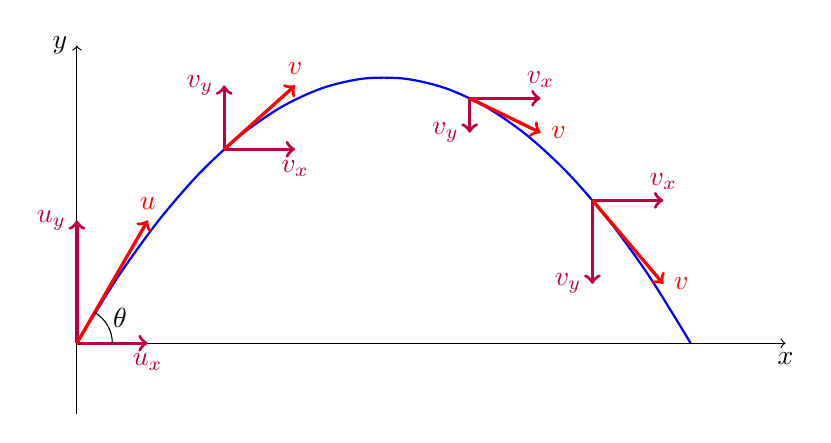
\begin{tikzpicture}[scale=.9]
	\draw[->] (0,-1) -- (0,4.2) node[left]{$y$};
	\draw[->] (0,0) -- (10,0) node[below]{$x$};
	\draw [thick,blue,domain=0:5*sqrt(3),samples=16,smooth,variable=\x] plot (\x,{sqrt(3)*\x-\x*\x/5});
	\draw[->,purple,very thick] (0, 0) -- ++(1,0) node[below]{$u_x$};
	\draw[->,purple,very thick] (0,0) -- ++(0,1.732) node[left]{$u_y$};
	\draw[->,red,very thick] (0,0) -- ++(1,1.732) node[above]{$u$};
	\foreach \idx in {1.2}
	{
		\draw[->,purple,very thick] (1.732*\idx, 3*\idx-.6*\idx*\idx) -- ++(1,0) node[below]{$v_x$};
		\draw[->,purple,very thick] (1.732*\idx, 3*\idx-.6*\idx*\idx) -- ++(0,1.732-0.693*\idx) node[left]{$v_y$};
		\draw[->,red,very thick] (1.732*\idx, 3*\idx-.6*\idx*\idx) -- ++(1,1.732-0.693*\idx) node[above]{$v$};
	}
	\foreach \idx in {3.2,4.2}
	{
		\draw[->,purple,very thick] (1.732*\idx, 3*\idx-.6*\idx*\idx) -- ++(1,0) node[above]{$v_x$};
		\draw[->,purple,very thick] (1.732*\idx, 3*\idx-.6*\idx*\idx) -- ++(0,1.732-0.693*\idx) node[left]{$v_y$};
		\draw[->,red,very thick] (1.732*\idx, 3*\idx-.6*\idx*\idx) -- ++(1,1.732-0.693*\idx) node[right]{$v$};
	}
	\draw (0.5,0) arc(0:60:0.5);
	\node at (30:0.7) {$\theta$};
	\end{tikzpicture}
	\caption*{components of the velocity of a projectile at different points along its path}
\end{figure}

\cmt horizontally, projectile maintains a constant velocity, so
\begin{equation*}
v_x = u_x \qquad x=u_x t
\end{equation*}

where $u_x = u\cos\theta$ is horizontal component of initial velocity

\cmt vertically, if upward direction is taken to be positive, then acceleration $a=-g$, so
\begin{equation*}
v_y = u_y + at = u_y - gt  \qquad y = u_y t + \frac{1}{2}at^2 = u_y t - \frac{1}{2}gt^2
\end{equation*}

where $u_y = u\sin\theta$ is vertical component of initial velocity

\cmt components can be combined to give resultant velocity or resultant displacement:
\begin{equation*}
 v = \sqrt{v_x^2 + v_y^2} \qquad s = \sqrt{x^2 + y^2}
\end{equation*}


\subsubsection*{maximum height reached by an projectile}

when a projectile reaches the highest position, its instantaneous vertical velocity becomes zero

we can then find the time it takes to attain this maximum height.
\begin{equation*}
	v_y = u\sin\theta - gt = 0 \RA t = \frac{u\sin\theta}{g}
\end{equation*}
	
to find $H_\tmax$, one can use either equation \eqref{eqn:const_a_eq2} or \eqref{eqn:const_a_eq3} 
	\begin{equation*}
	H_\tmax = \frac{1}{2}(u_y+v_y) t = \frac{1}{2}u_y t = \frac{1}{2} \times u \sin\theta \times \frac{u\sin\theta}{g} = \frac{u^2 \sin^2\theta}{2g}
	\end{equation*}
	\begin{equation*}
	H_\tmax = u_y t - \frac{1}{2}gt^2 = u \sin\theta \times \frac{u\sin\theta}{g} - \frac{g}{2} \times \left(\frac{u\sin\theta}{g}\right)^2 = \frac{u^2 \sin^2\theta}{2g}
	\end{equation*}

\cmt for the same initial speed $u$, the greater the angle of projection, the higher the object can get

in the extremal case where $\theta = 90 ^\circ$, it simply becomes an upward projection motion

\subsubsection*{airborne time and horizontal range of an projectile}

a ball projected from the ground will first rise in height

but it will eventually fall to the ground due to the gravitational pull after a period of time $T$

when it lands, its vertical displacement is zero, so
	\begin{equation*}
	Y = u_y T - \frac{1}{2}gT^2 = u \sin \theta T - \frac{1}{2}gT^2 = 0 \RA T = \frac{2u\sin\theta}{g}
	\end{equation*}
	
the horizontal range is given by
	\begin{equation*}
	X = u_x T = u\cos\theta \times \frac{2u\sin\theta}{g} = \frac{2u^2\sin\theta\cos\theta}{g} \RA X = \frac{u^2\sin2\theta}{g}
	\end{equation*}
	
where in the last step the trigonometric identity $\sin2\alpha = 2\sin\alpha\cos\alpha$ has been used

\cmt for same initial speed $u$, projectile launcher at greater angle stays in air for longer time

greatest airborne time is obtained if object is projected straight up, i.e.,  $\theta =90^\circ$

\cmt for same initial speed, horizontal range of projectile depends on angle $\theta$ of projection

to obtain the greatest horizontal range, two things are required

\titem sufficiently large horizontal velocity $v_x$

\titem sufficiently long time $T$ staying in the air

however, a larger $v_x$ requires a smaller $\theta$, hence a shorter airborne time $T$

therefore, there is a compromise between the two

optimal angle should be neither be too large nor too small, which can be shown to be $45^\circ$




\begin{figure}[ht]
	\centering
	\begin{tikzpicture}[scale=1]
	\draw[<->] (0,5.4) node[left]{$y$} -- (0,0) -- (11,0) node[below]{$x$};
	\draw [thick,red,domain=0:10,samples=16,smooth,variable=\x,graphlabel={[above]{$45^\circ$}}] plot (\x,{\x-0.1*\x*\x});
	\draw [thick,purple,domain=0:5*sqrt(3),samples=16,smooth,variable=\x,graphlabel={[above]{$60^\circ$}}] plot (\x,{sqrt(3)*\x-\x*\x/5});
	\draw [thick,purple,domain=0:5*sqrt(3),samples=16,smooth,variable=\x,graphlabel={[above]{$30^\circ$}}] plot (\x,{\x/sqrt(3)-\x*\x/15});
	\draw [thick,blue,domain=0:5,samples=16,smooth,variable=\x,graphlabel={[above]{$75^\circ$}}] plot (\x,{3.732*\x-\x*\x/1.34});
	\draw [thick,blue,domain=0:5,samples=16,smooth,variable=\x,graphlabel={[above]{$15^\circ$}}] plot (\x,{0.268*\x-\x*\x/18.66});
	\end{tikzpicture}
	\caption*{trajectories of projectiles launched at the same speed but different angles}\label{fig:projectile_range}
\end{figure}


\example{A ball is thrown from a point $O$ at $15 \mps$ at an angle of $40^\circ$ to the horizontal. The ball reaches its highest position at point $P$. Ignore the effects of air resistance. (a) How long does it take to reach $P$? (b) What is the magnitude of the displacement $OP$?}
		
\sol at highest point: $v_y = u_y - gt = 0 \RA t = \frac{u\sin\theta}{g} = \frac{15\times\sin40^\circ}{9.81} \approx 0.983 \text{ s}$

vertical displacement: $y = u_y t - \frac{1}{2}gt^2 = 15\sin40^\circ \times 0.983 - \frac{1}{2}\times 9.81 \times 0.983^2 \approx 4.74 \text{ m}$

horizontal displacement: $x = u_x t = 15\cos40^\circ \times 0.983 \approx 11.3 \text{ m}$

resultant displacement: $|OP| = \sqrt{x^2 +y^2} = \sqrt{11.3^2 + 4.74^2} \approx 12.2 \text{ m}$ \eoe

\newpage

\example{A small object is horizontally projected at 7.20 ms$^{-1}$ from a surface at a height of $h=1.2 \text{ m}$ above the ground. Assume there is no air resistance. (a) What is the time taken for the object to hit the ground? (b) What is the horizontal range? (c) Find the velocity at which the object hits the ground.}

\sol vertically, take downward as positive: $h = \cancelto{0}{u_y t} + \frac{1}{2}gt^2 \ra t = \sqrt{\frac{2h}{g}} = \sqrt{\frac{2\times1.2}{9.81}} \approx 0.495 \text{ s} $

horizontal range: $x = u_x t = 7.20 \times 0.495 \approx 3.56 \text{ m}$

final vertical velocity: $v_y = \cancelto{0}{u_y} + gt = 9.81 \times 0.495 \approx 4.85 \mps$

magnitude of resultant velocity: $v = \sqrt{v_x^2 + v_y^2} = \sqrt{7.20^2 + 4.85^2} \approx 8.68 \mps$

angle to which resultant velocity makes with horizontal: $\phi = \tan^{-1}\frac{v_y}{v_x} = \tan^{-1}\frac{4.85}{7.20} \approx 34^\circ$ \eoe


\ifthenelse{\includequestions=1}{

\subsection{end-of-chapter questions}

\subsubsection*{kinematic quantities}

\question{What is the distance covered for a car that travels half a lap along a circular path of radius of 200 m. What about the displacement?}

\question{A ball is released from a height of 2.0 m above the ground. It bounces vertically for quite a number of times before coming to rest. (a) State the change of displacement for the ball. (b) Explain how the distance travelled is different from the change in displacement.}


\question{For an athlete running around a track for many laps, suggest how his average velocity could be zero?}

\question{A car travels 2400 m east in 3.0 minutes, then takes a left turn, and then travels 700 m north in 1.5 minutes. What is the average speed and the average velocity for this journey?}

\question{Is it possible for an object moving at a steady speed to have acceleration?}


\subsubsection*{motion graphs}

\question{For the $v$-$t$ graph given in Example \ref{ex-vgraph}, sketch the $a$-$t$ graph for this motion.}

\question{If the tangent of a displacement-time graph at one particular instant is sloping downwards, what does that imply about the velocity at that instant?}

\question{A vehicle initially travels at a steady speed of $15 \mps$. It accelerates uniformly for 10 s to reach a higher speed of $20 \mps$. It maintains at this speed for 20 s, and then decelerates uniformly to a stop in the last 10 s. (a) Sketch the velocity-time graph for this motion. (b) Sketch the acceleration-time graph. (c) Find the distance travelled during the 40 s.}


\subsubsection*{linear motion with constant velocity}

\question{Sonar is a technique that uses sound waves to detect objects. It can be used to measure the depth of the seabed. Given that speed of sound in water is $1500 \mps$, and reflected waves sent from a submarine are detected 0.50s after they are transmitted. How deep is the water below the submarine?}

\question{Given that the speed of sound in air is $340 \mps$ and the speed of light in air is $3.0\times10^8 \mps$. If a person hears the sound of a thunder 5.0 seconds after seeing a lightning flash, how far away from this person is did the lightning strike?}



\subsubsection*{linear motion with constant acceleration}


\question{A train initially travels at a speed of $40\mps$. It starts to decelerate at 0.50\mpss. (a) What is the distance travelled in 50 s? (b) When it comes to a stop, how far out has it travelled?}

\question{A vehicle moving at $14\mps$ accelerate uniformly to $26\mps$ in 6.0 s. (a) What is the average velocity during this time? (b) What is the acceleration during this time (c) What is the distance travelled by the vehicle? (d) The vehicle then braked with constant deceleration to stop in another 8.0 s. What is the distance travelled during the time when brakes are applied?}


\subsubsection*{free fall}


\question{Two balls are dropped from rest from the same height. The second ball is released 0.80 s after the first one. What is their separation 1.5 s after the second ball is dropped?}

\question{A golf ball is dropped from the top of a tower of height 30 m. The ball falls from rest and air resistance is negligible. What time is taken for the ball to fall (a) the first 10 m from rest, (b) the last 10 m to the ground?}

\question{The acceleration of free fall on Pluto is about one-fifteenth of that on Earth. If it takes a time of $T$ for a rock to fall from rest a distance of $S$, what is the time taken, in terms of $T$, for a rock to fall from rest through the same distance $S$ on Pluto?}

\question{In an experiment is carried out to determine the acceleration of free fall $g$ using a falling body. The body is released from rest from a height of $h$, the time taken $t$ for it to hit the floor is measured. (a) Find the expression that can be used to calculate the value of $g$? (b) Suggest what could lead to an overestimation for the value of $g$.}


\subsubsection*{upward projection}

\question{A ball is tossed upwards with a speed of $9.0 \mps$. (a) How long does it take to return to the same point if air resistance is negligible? (b) How does the return velocity compare with its initial velocity?}

\question{Someone wants to toss a ball onto a platform that is at a height of 20 m above him. What is the minimum initial velocity needed to launch the ball?}

\question{Someone standing at the top of a high building throws a ball straight up and another ball straight down with the same initial speed. Assume that air drag is negligible, which ball will have a greater speed when it hits the ground?}

\question{In basketball games, hang time refers to the length of time a player stays in the air after jumping from the floor. (a) It is reported that Michael Jordan is able to stay in the air for $T=1.0\text{ s}$ to do his slam-dunk tricks, estimate how high he can jump. (b) The acceleration of fee fall on the Moon is about one-sixth of that on Earth. What is the hang time of Michael Jordan if he takes off from the surface of the Moon?}


\begin{wrapfigure}{r}{0.44\textwidth}
	\centering
	\vspace*{-10pt}
	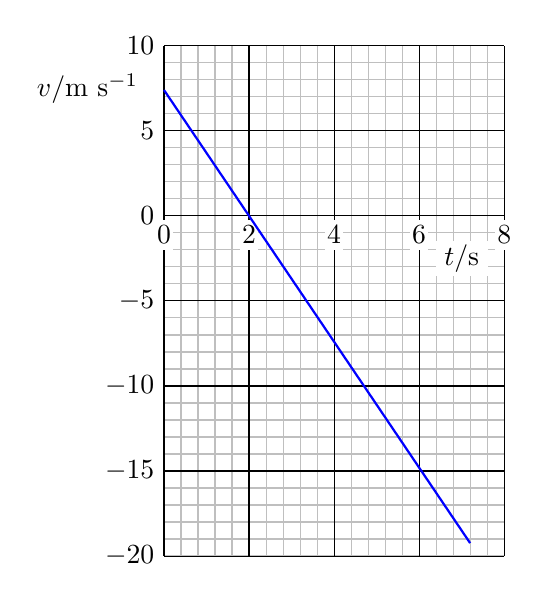
\begin{tikzpicture}[scale=1.08]
	\draw[thin, gray!50,step=0.2] (0,-4) grid (4,2);
	\draw[step=1] (0,-4) grid (4,2);
	\foreach \y in {10,5,...,-20} \node[left] at (0,\y/5){$\y$};
	\foreach \x in {0,2,...,8} 
	{
		\draw[white,fill] (\x/2-0.1,-0.4) rectangle (\x/2+0.1,-0.05);
		\node[below] at (\x/2,0) {$\x$};
	}
	\draw[thick,blue,domain=0:3.6] plot (\x, 1.48-1.48*\x); 
	\node at (-0.9,1.5) {$v$/m s$^{-1}$};
	\draw[white,fill] (3.2,-0.7) rectangle (3.8,-0.3);
	\node at (3.5,-0.5) {$t$/s};
	\end{tikzpicture}
	\vspace*{-15pt}
\end{wrapfigure}

\question{Mark Watney\footnote{A fictional character in the science fiction movie \emph{The Martian} (2015) based on the novel of the same name written by \emph{Andy Weir}.} stands at the edge of a cliff on the Mars and throws a rock vertically upwards with a speed of $7.4 \mps$. The graph shows the variation with the time $t$ of the rock's velocity $v$. (a) What is the acceleration of free fall on the Mars? (b) When does the rock reach the maximum height? (c) What is the height above the base of the cliff the moment when the rock is thrown? (d) What is the maximum height above the base of the cliff to which the rock rises? (e) What is the total distance travelled by the rock before it strikes the ground?}

\subsubsection*{projectile motion}

\question{A ball rolls off a table and lands at a position of a horizontal distance of 1.2 m from the table. The table is 0.95 m high. Find the speed at which the ball leaves the table.}

\question{A ball is kicked from the ground towards a vertical barrier. The barrier is at a horizontal distance of 18 m from the initial position of the ball. The ball strikes the barrier after 1.5 s at a height of 2.5 m above the ground. (a) Find the magnitude and the direction of the initial velocity. (b) Find the magnitude and the direction of the velocity at which the ball hits the barrier.}

\question{When a particle is launched from the origin at an angle $\theta$ with the horizontal at a speed of $u$, show that its trajectory is a parabola given by the equation: $y = x \tan\theta - \frac{gx^2}{2u^2\cos^2\theta}$.}\label{Q-projectile-eqn}

\question{Two golf players each hit a ball at the same speed. One at $30^\circ$ with the horizontal, the other at $60^\circ$. Which ball hits the ground first? Which ball goes farther?}

\question{(a) State the difference between the displacement of a projectile and the distance it travels. (b) Suggest in what situation a projectile's displacement could have the same magnitude as the distance.}

\question{An archer always aims slight higher than the distant target that she wants to hit. Why isn't the bow lined up such that it points exactly at the target?}


}{}